\documentclass[14pt]{extarticle} % zmienić na 14 przed wyslaniem tj
 
\usepackage[T1]{fontenc}
\usepackage[utf8]{inputenc}

\usepackage[hidelinks]{hyperref}

\usepackage{microtype}

\usepackage{amssymb}
\usepackage{amsmath}
\usepackage{mathtools}
\usepackage{dsfont}

\usepackage{enumitem}

\usepackage{tikz}
\usetikzlibrary{cd, patterns, patterns.meta, decorations.pathmorphing}

\usepackage{geometry}
\geometry{a4paper, total={170mm, 252mm}, top=22mm}

\usepackage[skip=7pt]{parskip}

\usepackage{amsthm}
\usepackage{thmtools}

\newtheoremstyle{straightstyle}
  {6pt} % Space above
  {6pt} % Space below
  {} % Body font
  {} % Indent amount
  {\bfseries} % Theorem head font
  {.} % Punctuation after theorem head
  {.5em} % Space after theorem head
  {} % Theorem head spec (can be left empty, meaning `normal')

\newtheoremstyle{italicsstyle}
  {6pt} % Space above
  {6pt} % Space below
  {\slshape} % Body font
  {} % Indent amount
  {\bfseries} % Theorem head font
  {.} % Punctuation after theorem head
  {.5em} % Space after theorem head
  {} % Theorem head spec (can be left empty, meaning `normal')

\declaretheorem[ %
  name=Definition, %
  numberwithin=section, %
  style=italicsstyle
]{definition}

\declaretheorem[ %
  name=Theorem, %
  numberwithin=section, %
  style=straightstyle
]{theorem}

\declaretheorem[ %
  name=Proposition, %
  numberlike=theorem, %
  style=straightstyle
]{proposition}

\declaretheorem[ %
  name=Corollary, %
  numberlike=theorem, %
  style=straightstyle
]{corollary}

\declaretheorem[ %
  name=Lemma, %
  numberlike=theorem, %
  style=straightstyle
]{lemma}

\declaretheorem[ %
  name=Remark, %
  numberlike=definition, %
  style=italicstyle
]{remark}

\declaretheorem[ %
  name=Example, %
  numberwithin=section, %
  style=straightstyle
]{example}


% \renewenvironment{proof}{{\bfseries Proof}$ $\newline}{
%   \begin{flushright} $ \spadesuit $ \end{flushright}$ $\newline
% }

\usepackage{cleveref}

%\crefname{definition}{definicja}{definicje}
%\Crefname{definition}{Definicja}{Definicje}
%
%\crefname{theorem}{twierdzenie}{twierdzenia}
%\Crefname{theorem}{Twierdzenie}{Twierdzenia}
%
%\crefname{lemma}{lemat}{lematy}
%\Crefname{lemma}{Lemat}{Lematy}
%
%\crefname{remark}{uwaga}{uwagi}
%\Crefname{remark}{Uwaga}{Uwagi}


\DeclareMathOperator{\Z}{\mathbb{Z}}
\DeclareMathOperator{\R}{\mathbb{R}}
\DeclareMathOperator{\C}{\mathbb{C}}
\DeclareMathOperator{\N}{\mathbb{N}}
\DeclareMathOperator{\Q}{\mathbb{Q}}

\DeclareMathOperator{\im}{im}
\DeclareMathOperator{\coker}{coker}

\newcommand{\set}[1]{\mathcal{#1}}


\DeclareMathOperator{\ord}{ord}
\DeclareMathOperator{\Ann}{Ann}
\DeclareMathOperator{\Hom}{Hom}

\DeclareMathOperator{\Col}{Col}

\DeclareMathOperator{\End}{End}

\let\landtemp\land
\renewcommand{\land}{\;\landtemp\;}





\usepackage{tikz}
\usetikzlibrary{spath3, hobby, knots, braids}

\pgfdeclarelayer{bg}    % declare background layer
\pgfsetlayers{bg,main}

% Fox colorings and Alexander invariants
\title{ {\bfseries Knot colorings and homological invariants}\\ \medskip {\normalsize(Kolorowania węzłów i niezmienniki homologiczne.)}}
\author{
  Weronika Jakimowicz\\
  330006
}
\date{\medskip Praca licencjacka 2023-2024}

% \definecolor{red}{HTML}{000000}
% \definecolor{blue}{HTML}{000000}
% \definecolor{orange}{HTML}{000000}
% \definecolor{green}{HTML}{000000}

% \includeonly{rozdzialy/04-00-category.tex}
% \includeonly{wstep.tex}
% \includeonly{rozdzialy/01-00-preliminaries.tex}

\begin{document}
\maketitle
\bigskip

\begin{center}
  \large
  \textbf{Promotor:} prof. Tadeusz Januszkiewicz
\end{center}
\vspace{10pt}

\begin{center}
\scalebox{0.7}{
    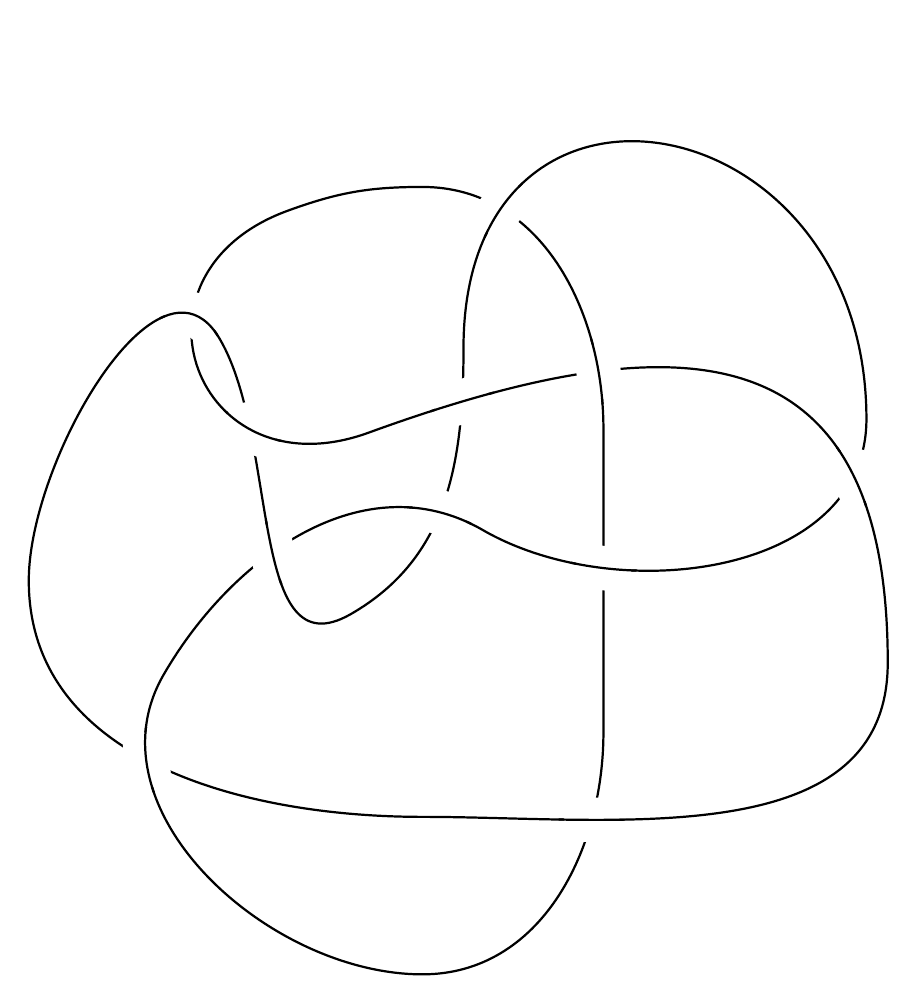
\begin{tikzpicture}
      \coordinate (a1) at (90:5);
      \coordinate (a2) at (40:3);
      \coordinate (a3) at (-40:3);
      \coordinate (a4) at (-90:5);
      \coordinate (a5) at (-160:3.5);
      \coordinate (a6) at (40:1);
      \coordinate (a7) at (20:6);
      \coordinate (a8) at (80:3);
      \coordinate (a9) at (180+25:1);
      \coordinate (a10) at (130:4);
      \coordinate (a11) at (180:5);
      \coordinate (a12) at (-90:3);
      \coordinate (a13) at (-10:6);
      \coordinate (a14) at (110:2);
      \coordinate (a15) at (110:5);

      % \foreach \i in {1,..., 15} \fill (a\i) circle (5pt);

      \begin{knot}[
        consider self intersections, 
        clip width = 20pt, 
        % draft mode=crossings, 
        flip crossing=1, 
        flip crossing=3, 
        flip crossing=8, 
        flip crossing=4, 
        flip crossing=7, 
        flip crossing=10, 
        flip crossing=9
        ]
        \strand[thick] (a1) to[out=0, in=90] 
        (a2) to[out=-90, in=90] 
        (a3) to[out=-90, in=0] 
        (a4) to[out=180, in=-120]
        (a5) to[out=60, in=150]
        (a6) to[out=-30, in=-90] 
        (a7) to[out=90, in=90, looseness=2] 
        (a8) to[out=-90, in=30]
        (a9) to[out=-150, in=-60]
        (a10) to[out=120, in=90] 
        (a11) to[out=-90, in=180]
        (a12) to[out=0, in=-90] 
        (a13) to[out=90, in=20, looseness=1.5]
        (a14) to[out=-160, in=200, looseness=2]
        (a15) to[out=20, in=180] 
        (a1);
      \end{knot}
    \end{tikzpicture}
    % \caption{A diagram for knot $K11n164$.\label{k11n164 diagram}}
}
\end{center}

% \begin{center}
%   \begin{tikzpicture}[bgnd/.style={circle, fill=white, draw=white}]
%     %\node[opacity=0.2] at (0,0) {\includegraphics[width=0.7\textwidth]{./rozdzialy/6_1-3d.png}};
%
%     \coordinate (a0) at (0,0);
%     \coordinate (a1) at (90:5);
%     \coordinate (a2) at (45:3);
%     \coordinate (a3) at (-40:4.6);
%     \coordinate (a4) at (-120:2.4);
%     \coordinate (a5) at (10:0.7);
%     \coordinate (a6) at (50:5);
%     \coordinate (a7) at (90:3.5);
%     \coordinate (a8) at (180-50:5);
%     \coordinate (a9) at (170:0.7);
%     \coordinate (a10) at (-70:2.4);
%     \coordinate (a11) at (220:4.6);
%     \coordinate (a12) at (180-45:3);
%
%     %\foreach \i in {0,...,12} \fill (a\i) circle (2pt);
%
%     \begin{knot}[
%       clip width=20,
%       flip crossing=1,
%       flip crossing=3,
%       flip crossing=6
%       ]
%       \strand[thick] (a1) to[out=0, in=90+45] (a2) to[out=-45, in=40] (a3);
%       \strand[thick] (a3) to[out=220, in=-90] (a4) to[out=90, in=200] (a5);
%       \strand[thick] (a5) to[out=20, in=-30] (a6);
%       \strand[thick] (a6) to[out=150, in=5] (a7);
%       \strand[thick] (a7) to[out=175, in=30] (a8);
%       \strand[thick] (a8) to[out=210, in=160] (a9);
%       \strand[thick] (a9) to[out=-20, in=90] (a10);
%       \strand[thick] (a10) to[out=-90, in=-40] (a11);
%       \strand[thick] (a11) to[out=140, in=180+45] (a12);
%       \strand[thick] (a12) to[out=45, in=180] (a1);
%     \end{knot}
%   \end{tikzpicture}
% \end{center}

\newpage

\section*{Abstract}

The knot group $G=\pi_1(K)$ is a starting point for many knot invariants. Alexander matrix is a representation matrix for a subgroup of $G$ and from its determinant, the Alexander polynomial is obtained. Another way of obtaining said polynomial is by considering a coloring matrix which assigns elements of $R$-module $M$ to segments from a diagram $D$ of knot $K$. This approach can be derived from the image of a resolution of Alexander module through the functor $\Hom(-, M)$. Nevertheless, color checking matrices do not instantly yield a knot invariant, however it is possible to define an equivalence relation that identifies matrices stemming from the same knot. This approach is used to distinguish a pair of knots with the same Alexander polynomial. In the end, a way of generalizing the procedure of coloring diagrams is presented in terms of category theory.

\section*{Introduction}

\Cref{sec1} defines the fundamental ideas of this paper, such as the knot group (see \cref{knot gorup def}) its metabelianization (see \cref{def:metabelianization}) and the Alexander module (see \cref{alexander module def}). Two equivalent definitions fot said modules are presented: an algebraic one and a topological one. In a purely algebraical sense, the Alexander moule is the abelianized subgroup $[[G, G], [G, G]]$ of the knot group $G$, with $\Z$ action induced by abelianization homomorphism $G\to \Z$, while from a topological point of view it is the first homology module of the infinite cyclic cover (see \cref{inf cyclic cover}). An important result finishing this section is that the Alexander module is a torsion module (see \cref{prop: modul alexandera jest torsyjny}).

\Cref{section2} is dedicated to the Alexander matrix (see \cref{alexander matrix def}) its properties and ivariant nature of its determinant.




\newpage

\tableofcontents

\newpage

\section{Preliminaries}\label{sec1}

\subsection{Knots and diagrams}

In mathematical terms, a knot is a smooth embedding $S^1\hookrightarrow S^3$. A knot diagram is an {immersive projection} $D:S^1\hookrightarrow \R^2$ along a vector such that no three points of the knot lay on this vector \cite{likorish-diagram}. If two points are mapped to one by this projection, we say that a small neighbourhood of this point which looks locally like \begin{tikzpicture}\draw(-.5ex,0)--(2.5ex, 0ex); \fill[white](1ex, 0) circle (.5ex);\draw(1ex, -1ex)--(1ex, 1ex);\end{tikzpicture} is a crossing.

% $S^1$ is an orientable space thus we can choose an orientation for a knot being considered. Then a diagram $D$ is oriented if it is a projection of an oriented $S^1$.

$S^1$ is orientable, thus we can chose an orientation for any knot and, as a consequence, its diagram.

Intuitively, two knots $K_1$ and $K_2$ are equivalent if we can deform one into the other
%without cutting it and only manipulating it with our hands 
\cite{murasagi-equivalence}. This translates to an equivalence of diagrams, which is generated by comparing diagrams that are exactly the same save for an interior of some disc in $R^2$. If inside of said disc the diagrams differ by one of \buff{Reidemeister moves}, we say that they are equivalent. 
%
% This translates to equivalence of diagrams, which is generated by a set of moves, called the \buff{Reidemeister moves}. 
%
In the case of a diagram without an orientation, three moves are sufficient. When an orientation is imposed on $D$, $4$ diagram moves (pictured in \cref{reidemeister-generating}) generate the whole equivalence relation \cite{ruchy_zorientowane}.

\begin{figure}[h]\centering
  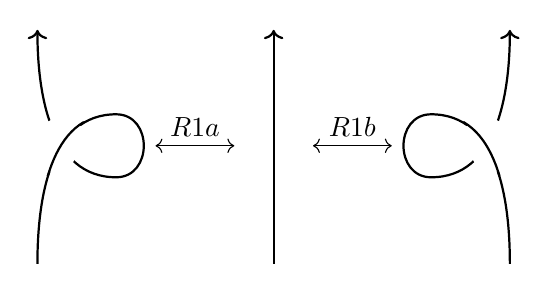
\begin{tikzpicture}
    \begin{knot}[
      consider self intersections, 
      clip width=20pt, 
      %draft mode=crossings,
      flip crossing=4,
      flip crossing=3,
      ]
      \strand[->, thick] (0, 0) to [out=90, in=180] 
      (1, 1.9) to [out=0, in=0, looseness=1.5] 
      (1, 1.1) to[out=180, in=-90] (0, 3);
      \strand[->, thick] (3, 0)--(3, 3);
      \strand[->, thick] (6, 0) to[out=90, in=0] 
      (5, 1.9) to[out=180, in=180, looseness=1.5]
      (5, 1.1) to[out=0, in=-90] (6, 3);
    
    \end{knot}
    \draw[<->] (1.5, 1.5)--(2.5, 1.5) node[midway, above] {$R1a$};
    \draw[<->] (3.5, 1.5)--(4.5, 1.5) node[midway, above] {$R1b$};

  \end{tikzpicture}
  \vspace{1cm}

  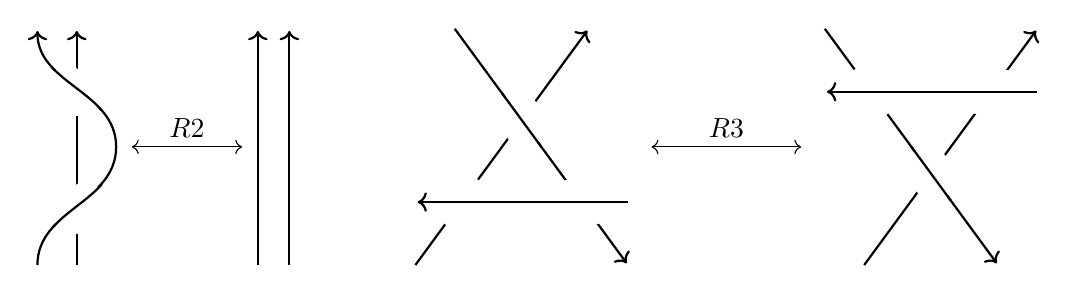
\begin{tikzpicture}
    \begin{knot}[
      consider self intersections, 
      clip width=20pt, 
      %draft mode=crossings, 
      flip crossing=2, 
      flip crossing=1, 
      flip crossing=3, 
      flip crossing=4, 
      flip crossing=5,
      flip crossing=6, 
      flip crossing=8, 
      flip crossing=7
      ]
      \strand[->, thick] (1.8, -5)--(1.8, -2);
      \strand[->, thick] (2.2, -5)--(2.2, -2);

      \strand[->, thick] (-.5, -5)--(-.5, -2);
      \strand[->, thick] (-1, -5) to[out=90, in=-90] 
      (0, -3.5) to[out=90, in=-90] 
      (-1, -2);

      \strand[->, thick] (3.8, -5)--(6, -2);
      \strand[->, thick] (4.3, -2)--(6.5, -5);
      \strand[<-, thick] (3.8, -4.2)--(6.5, -4.2);

      \strand[->, thick] (9.5, -5)--(11.7, -2);
      \strand[->, thick] (9, -2)--(11.2, -5);
      \strand[<-, thick] (9, -2.8)--(11.7, -2.8);
    \end{knot}
    
    \draw[<->] (.2, -3.5) -- (1.6, -3.5) node[midway, above] {$R2$};

    \draw[<->] (6.8, -3.5)--(8.7, -3.5) node[midway, above] {$R3$};
  \end{tikzpicture}
  \caption{Generating set of Reidemeister moves in oriented diagrams. \label{reidemeister-generating}}
\end{figure}


\subsection{Knot group}

Let $K$ be a knot and $D$ be its oriented diagram with $s$ segments and $x$ crossings. 
%A crossing of a diagram is a point in projection $S^1\to \R^2$ with exactly two points in its preimage along with a small neighbourhood that looks locally like \begin{tikzpicture}\draw(-.5ex,0)--(2.5ex, 0ex); \fill[white](1ex, 0) circle (.5ex);\draw(1ex, -1ex)--(1ex, 1ex);\end{tikzpicture}. 
A segment of a diagram is a line of the diagram between two crossings in which it is disappears under another line.

%The knot itself has the homotopy type of a circle and so its fundamental group is not interesting in itself. However, for a knot that is embedded in $S^3$ we can study the fun
\begin{definition}[knot group] 
  The fundamental group of knot complement $X=S^3-K$  is called a \buff{knot group}:
  \boldmath$$\mathbf{\pi_1(K):=\pi_1(X)}.
  $$
\end{definition}
Although the knot itself is always a circle $S^1$, the knot group has usually an interesting yet difficult structure. The most commonly used presentation of the knot group is called \buff{the Wirtinger presentation}.

\begin{definition}[Wirtinger presentation]
  Given a diagram $D$ of knot $K$ with segments $a_1$, $a_2$, ..., $a_s$ and crossings $c_1$, ..., $c_x$ the knot group $\pi_1(K)$ can be represented as $\pi_1(K)=\langle G\;|\;R\rangle$, where $G$ is the set of segments of $D$ and relations $R$ correspond to crossings in the manner described in the diagram below
  \begin{center}
    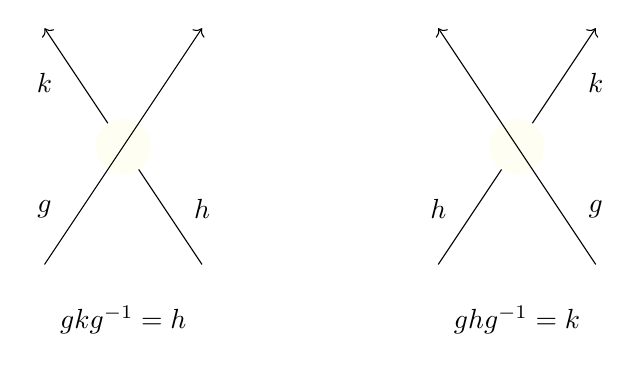
\begin{tikzpicture}
      \begin{scope}
        \draw[->] (2, 0)--(0, 3);
        \fill[yellow!5] (1, 1.5) circle (10pt);
        \draw[->] (0, 0)--(2, 3);
        \node at (0, .7) {$g$};
        \node at (0, 2.3) {$k$};
        \node at (2, .7) {$h$};

        \node at (1, -.7) {$gkg^{-1}=h$};
      \end{scope}

      \begin{scope}[shift={(5, 0)}]
        \draw[->] (0, 0)--(2, 3);
        \fill[yellow!5] (1, 1.5) circle (10pt);
        \draw[->] (2, 0)--(0, 3);
        \node at (0, .7) {$h$};
        \node at (2, 2.3) {$k$};
        \node at (2, .7) {$g$};
        
        \node at (1, -.7) {$ghg^{-1}=k$};
      \end{scope}
    \end{tikzpicture}
  \end{center}
  Representation $\langle G\;|\;R\rangle$ described above is called the \buff{Wirtinger presentation} \cite[Chapter~6]{livingstone}.
\end{definition}

An easily obtainable result, either by applying the Mayer-Vietoris sequence to $S^3=K\oplus S^3-K$ or noticing that every two generators are conjugate, is that the abelianization of the knot group is always $\Z$. This leads to a short exact sequence
\begin{center}
  \begin{tikzcd}
    0\arrow[r] & K_G \arrow[r] & G=\pi_1(K)\arrow[r, "ab"] & \Z=G^{ab} \arrow[r] & 0.
  \end{tikzcd}
\end{center}

The group $K_G=\ker(ab:G\to\Z)=[G, G]$ in general is not abelian nor finitely generated, an observation that is discussed in \cref{alexander module discussion}, and thus is a difficult group to work with. However, its abelianization $K_G^{ab}=K_G/[K_G, K_G]$ allows a $\Z[\Z]$ module structure and thus contains obtainable information about the knot $K$. 

\begin{lemma}
  For any group $G$, the commutator of its commutator $K_G$ is a normal subgroup: $[K_G, K_G]=[[G, G], [G, G]\triangleleft G$. 
\end{lemma}

\begin{proof}
  The commutator subgroup is a characteristic subgroup, since for any automorphism $\phi:G\to G$ 
  $$\phi(hgh^{-1}g^{-1})=\phi(h)\phi(g)\phi(h)^{-1}\phi(g)^{-1}\in K_G=[G, G].$$
  Conjugation by any element $g\in G$ is an automorphism of the commutator $K_G$. Thus it preserves its commutator subgroup $[K_G, K_G]$. 
\end{proof}

As a consequence, in the group $G/[K_G, K_G]$ left and right multiplication is the same. Thus, the following is an exact sequence:
\begin{center}
  \begin{tikzcd}
    0\arrow[r] & K_G^{ab} \arrow[r] & G^{mab}=G/[K_G, K_G]\arrow[r] & \Z \arrow[r] & 0
  \end{tikzcd}
\end{center}
which gives foundation for the following definition.

% If $G$ is considered in its Wirtinger presentation, then $K_G$ does not have a finite set of generators. If $a_1$,..., $a_s$ where the generators of $G$ such that $(a_i)^{ab}=1$ for every $i$, then choosing new generators to be $x_i=a_ia_1^{-1}$ for $i=2,..., s$ implies that $K$ is generated by $a_1^{k}x_ia_1^{-k}$ for $i=2,...,s$ and $k\in\Z$.

\begin{definition}[metabelianization]\label{def:metabelianization}
  The quotient group $G^{mab}=G/[K_G, K_G]$ is called the \buff{metabelianization} of $G$. 
\end{definition}

We will return to the concept of metabelianization in \cref{section2}. For the time being, let us assign a name to $K_G$:

\begin{definition}[Alexander module]\label{alexander module def}
  Given a group $G$, the abelianization of the commutator of a group $G$, $K_G^{ab}$, with $\Z[\Z]$-module structure is called the \buff{Alexander module} of $G$. If $G$ is a knot group, then it is the Alexander module of the knot $K$.
\end{definition}

How the $\Z[\Z]$ module structure is obtained is described in detail in \cref{alexander module discussion}.






\subsection{Infinite cyclic covering}

Let $X$ be the complement of a knot $K$, that is $X=S^3-K$. Take $\widetilde{X}$ to be its universal covering, meaning that its fundamental group is trivial. The fundamental group $G$ of $X$ acts on its universal covering by deck transformations. The commutator subgroup $K_G=[G, G]$ is normal in $G$ and so we the action of $K_G$ on $\widetilde{X}$ is well defined. Thus we might take the quotient space $\overline{X}=\widetilde{X}/[G, G]$ and call it the \buff{infinite cyclic covering} of $X$. The fundamental group of $\overline{X}$ is exactly 
$$\pi_1(\overline{X})=[G, G]=K_G$$
and from the perspective of homology modules, we have
$$H_1(\overline{X}, \Z)=\pi_1(\overline{X})^{ab}=K_G^{ab}.$$

The following diagram illustrates the construction described above

\def\actson{
  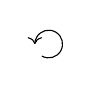
\begin{tikzpicture}[baseline]
    \draw[->](0, 0) arc (-120:180:.5em);
  \end{tikzpicture}
}

\begin{center}
  \begin{tikzcd}[column sep=tiny]
    \widetilde{X}\arrow[d] & \arrow[l, phantom, sloped, "\actson"] G \\ 
    \overline{X} \arrow[d] & \arrow[l, phantom, sloped, "\actson"] G/[K_G, K_G] \\ 
    X=S^3-K
  \end{tikzcd}
\end{center}

% \begin{lemma}
%   The following is a short exact sequence of chain complexes
%   \begin{center}
%     \begin{tikzcd}
%       0 \arrow[r] & C_*(\overline{X})\arrow[r, "t-1"] & C_*(\overline{X})\arrow[r] & C_*(X)\arrow[r] & 0 
%     \end{tikzcd}
%   \end{center}
% \end{lemma}
%

A \buff{Seifert surface} $S$ of knot $K$ is an orientable surface with boundary embedded in $S^3$ such that $\partial S=K$. Take a countable amount of $X$, with $S$ without its boundary embedded, and label each with an element from $\Z$. We might now cut each of the copies of $X$ along the Seifert surface of $K$ and identify the $+$ side of $S$ from the $i$-th copy of $X$ with the $-$ side of $S$ from the $(i+1)$-th copy of $X$. Notice that the arising space with a projection to one copy of $X$ is an infinite cyclic cover of $X$.

Imagine that each copy of $X$ inside of $\overline{X}$ is a box labeled with some integer $k$. The ring action of $\Z[\Z]$ on $\overline{X}$ is increasing or decreasing the label on the box from which a cycle is taken, depending on the power of $t\in\Z[\Z]$ in the polynomial which we apply to $\overline{X}$.

\begin{proposition}\label{prop: modul alexandera jest torsyjny}
  The $\Z[\Z]$-module $K^{ab}=H_1(\overline{X}, \Z)$ is a torsion module.
\end{proposition}

\begin{proof}
  Consider the following homomorphism on chain complexes:
  $$f:C_*(\overline{X})\to C_*(\overline{X})$$
  $$f(x)=(1-t)x.$$
  It translates to removing from a cycle in the $(i+1)$-th box a corresponding cycle in the $i$-th box. From this it is an immediate result that $\ker f=0$ and that $\coker f=C_*(X)$ : after gluing all pairs of cycles from two consecutive boxes, the result is easily identified with just one box.

  As a consequence, the following sequence of chain complexes is exact
  \begin{center}
    \begin{tikzcd}
      0\arrow[r] & C_*(\overline{X})\arrow[r, "f"] & C_*(\overline{X})\arrow[r] & C_*(X)\arrow[r] & 0
    \end{tikzcd}
  \end{center}
  and induces an acyclic complex of homology modules
  \begin{center}
    \begin{tikzcd}
      ... \arrow[r] & H_2(X, \Z)\arrow[r] & H_1(\overline{X}, \Z)\arrow[r, "1-t"] & H_1(\overline{X}, \Z)\arrow[r] & H_1(X, \Z)
      \arrow[dlll, rounded corners, to path={--([xshift=2ex]\tikztostart.east) |- ([xshift=-3ex, yshift=-2ex]\tikztostart.south) -| ([xshift=-2ex]\tikztotarget.west) -- (\tikztotarget)
      }]\\ 
                    & H_0(\overline{X}, \Z)\arrow[r] & H_0(\overline{X}, \Z)\arrow[r] & H_0(X, \Z)\arrow[r] & 0
    \end{tikzcd}
  \end{center}
  As was mentioned previously, the following equality holds:
  $$H_1(X, \Z)=\pi_1(X)^{ab}=\Z.$$
  Now, because $X$ is homotopy cycle, then $H_2(X, \Z)=0$. Both $X$ and $\overline{X}$ is connected implying that 
  $$H_0(X, \Z)=H_0(\overline{X}, \Z)=\Z.$$
  \begin{center}
    \begin{tikzcd}
      ... \arrow[r] & 0\arrow[r] & H_1(\overline{X}, \Z)\arrow[r, "1-t"] & H_1(\overline{X}, \Z)\arrow[r, "0"] & \Z \arrow[dlll, "\cong", rounded corners, to path={--([xshift=2ex]\tikztostart.east) |- ([xshift=-3ex, yshift=-2ex]\tikztostart.south) -| ([xshift=-2ex]\tikztotarget.west) -- (\tikztotarget)
      }]\\ 
                    & \Z \arrow[r, "0"] & \Z\arrow[r, "\cong"] & \Z \arrow[r] & 0
    \end{tikzcd}
  \end{center}
  Rewriting the sequence above we easily get that homomorphism $1-t$ is actually an isomorphism and $H_1(\overline{X}, \Z)\cong (1-t) H_1(\overline{X}, \Z)$, which allows us to use the Nakayama's lemma to conclude that there exists $x\in\Z[\Z]$ such that
  $$xH_1(\overline{X}, \Z)=0.$$
\end{proof}



\section{Resolution of the Alexander module}
\label{section2}

\subsection{Alexander module}
\label{alexander module discussion}

Take $G=\langle G\;|\;R\rangle$ to be the Wirtinger presentation of $G$ obtained from oriented diagram $D$. Because $K$ is a knot and not a link, we know that the number of segments is equal to the number of crossings, thus we can take $n=s=x$ \cite{julia_private}.

Let $a_1,...,a_n$ be the generators of $G$ and $x_1,...,x_n$ its relations. The homomorphism of abelianization of $G$ is defined by 
$$a_i\mapsto 1\in\Z$$ 
for every $i=1,...,n$. In order to obtain a presentation of $K_G$, the kernel of abelianization, we need to change the set of generators of $G$ to 
$$\{a_1, A_2=a_2a_1^{-1},..., A_n=a_na_1^{-1}\}.$$
It is obvious that for every $i>1$ $A_i\mapsto0$ by abelianization of $G$. Thus $A_2,...,A_n$ are some of the generators of $K_G$. However, for each $i=2,...,n$ and $k\in\Z$ the following is an element of $K_G$:
$$b_{i, k}:=a_1^k A_i a_1^{-k}.$$
Thus, the presentation of $K_G$ as an abelian group is infinite with (possibly redundant) generators 
$$\{b_{i,k}\;:\;i=2,...,n,\;k\in\Z\}.$$

Changing generators of $G$ induced a change in relations. Suppose that the following relation was true in $G$
$$a_k=a_ia_ja_i^{-1}.$$
If $1\notin\{i,k,j\}$ then after the change of generators the relation is
$$ A_ka_1 = A_ia_1 A_ja_1 (A_ia_1)^{-1}
$$
forcing each element to be a conjugate of $a_1$ the following two relations can be obtained
$$ a_1^{-1}A_ka_1=(a_1^{-1} A_i a_1)A_jA_i^{-1}
$$
$$
a_1^{-3} A_k a_1^3 = (a_1^{-3} A_i a_1^3) (a_1^{-2} A_j a_1^2) (a_1^{-2} A_i^{-1} a_1^2).
$$
Obviously in $G$ both of those relations are equivalent, however in $K_G$ they are distinct. Moreover, we can write 
$$
b_{k, x}=b_{i, x}b_{j, x-1}b_{i, x-1}^{-1}
$$
to obtain infinitely many relations from $K_G$.

It was mentioned in the previous chapter, that following is an exact sequence
\begin{center}
  \begin{tikzcd}
    0\arrow[r] & K^{ab}_G\arrow[r] & G^{mab}\arrow[r] & \Z\arrow[r] & 0.
  \end{tikzcd}
\end{center}
For any group $H$ with $H^{ab}=\Z$ we can write a homomorphism $\Z\to H$ such that composition $\Z\to H\to \Z$ is identity on $\Z$. Thus, this sequence splits and we can write 
$$G^{mab}=K^{ab}_G\rtimes \Z.$$ 
Hence action of $\Z$ can be defined on the group $K^{ab}_G$, with presentation described above, as follows 
$$t(b_{i, k})=b_{i, k+1}.$$
In particular, 
$$t(A_i)=a_1 A_i a_1^{-1}.$$
This procedure allows $K_G^{ab}$ to be interpreted as a $\Z[\Z]$-module.

Moreover, the group $G^{mab}$ and $\Z[\Z]$ $K_G^{ab}$ can be used interchangeably as knowing the action of $\Z$ on $K_G^{ab}$ allows us to write the semidirect product of $\Z$ and $K_G^{ab}$.

% {\color{blue}
% \begin{lemma}
%   The $\Z[\Z]$ modules $K_G^{ab}$ and $G^{mab}$ (see \cref{def:metabelianization}) are isomorphic.
% \end{lemma}
%
% \begin{proof}
%   Construction presented above states that the module $K_G^{ab}$ has $(n-1)$ generators.
% \end{proof}
% }

% Notice that if $G^m$ is known, one can easily reconstruct $K_G^{ab}$ knowing that it is the $\ker(G^m\to \Z)$. Conversely, if $K_G^{ab}$ is known, then $G^m$ can be found as the middle term of the exact sequence \begin{tikzcd}[column sep=small]0\arrow[r]& K_G^{ab}\arrow[r] &? \arrow[r] & \Z\arrow[r] & 0\end{tikzcd}






\subsection{Basic properties}

Knowing the resolution of a module allows one to change said module into a matrix or even a sequence of matrices, each containing at least a portion of information about its structure.
%at first glance is in no way a simplification of said module. However, there are multiple ways of distilling simplifications and invariants from the resolution of the Alexander module. 
% {\large\color{red}In this section we want to }

\begin{definition}[Alexander matrix]
  The presentation matrix $A_D$ of $K_G^{ab}$ with Wirtinger presentation is \hl{the matrix $\Z[\Z]^n\xrightarrow[A_D]{}\Z[\Z]^{n-1}$ such that $\ker(A_D)$ is equal to module of relations of $K_G^{ab}$.} This matrix is called the \buff{Alexander matrix} of the Alexander module $K_G^{ab}$.
\end{definition}

We start writing the beginning $K_G^{ab}$ resolution as follows:
\begin{equation}\label{pierwsza rezolwenta}
  \begin{tikzcd}
    ...\arrow[r] & \Z[\Z]^{n}\arrow[r, "A_D"] & \Z[\Z]^{n-1}\arrow[r] & K_G^{ab}\arrow[r] & 0
  \end{tikzcd}
\end{equation}


% \begin{definition}[Alexander matrix]\label{alexander matrixi def}
%   The matrix of homomorphism $A_D$ in the diagram above is called the \buff{Alexander matrix} of group $G$ (knot $K$).
% \end{definition}

The Alexander matrix in the case of a knot group is not a square matrix. However, striking out any of its columns will give a square matrix whose determinant is nonzero. We will prove this statement promptly after consider the Alexander module as a vector space over the field of fractions of $R=\Z[\Z]$ \cite[Chapter~3]{atiyah}.

In \cref{prop: modul alexandera jest torsyjny} it was shown that the Alexander module is torsion. Thus, as a vector space $K_G^{ab}\otimes_R R^{-1}R=0$ it is trivial. Hence, the sequence in (\ref{pierwsza rezolwenta}) translates to the following sequence of $R^{-1}R$ modules
\begin{equation}\label{resolution vector spaces}
  \begin{tikzcd}
    ...\arrow[r] & R^n\otimes_R R^{-1}R \arrow[r, "A_D^V"] & R^{n-1}\otimes_R R^{-1}R \arrow[r] & 0
  \end{tikzcd}
\end{equation}
As there exists an inclusion $R\hookrightarrow R^{-1}R$, every matrix with terms in $R$ can be treated as a matrix with terms in $R^{-1}R$. Naturally, $A_D^V=A_D\otimes Id_{R^{-1}R}$ is just matrix $A_D$ (with terms in $R$) with adjoined $1\times 1$ matrix with just identity of $R^{-1}R$. Thus, we can easily translate most properties of $A_D^V$ to properties of $A_D$, i.e. its determinant and surjectivity.%, by forgetting the $R^{-1}R$ factor.

\begin{proposition}\label{alexander matrix has trivial kernel}
  Let $A_D'$ be the Alexander matrix $A_D$ with one of its rows struck out. Then $\det(A_D')\neq 0$.
\end{proposition}

\begin{proof}
  % We will show that $\det(A_D')(1)=\pm1$.
  %
  We start by noticing that every crossing contains three segments and so every row of the Alexander matrix has at most three non-zero terms. The relation in Wirtinger presentation generated by crossing 
  \begin{center}
    \begin{tikzpicture}
      \draw(0,0)node[above]{$a$}--(2, 3) node[above] {$b$};
      \fill[white] (1, 1.5) circle (20pt);
      \draw[->](2, 0)--(0, 3) node[above] {$u$};
    \end{tikzpicture}
  \end{center}
  is of form
  $$ubu^{-1}=c.$$
  As described in the previous section, we change the Wirtinger presentation so that only one generator $x$ is send to $1$ by abelianization. If said generator is $u=x$, then in the $\Z[\Z]$ module $K^{ab}$ we see the following relation 
  $$\pm t^n(tB-C)=0,$$
  where $B=bx^{-1}$ and $C=cx^{-1}$. Otherwise, the relation is
  $$\pm t^n[(1-t)U+tB-C]=0,$$
  and the row corresponding to this crossing in the Alexander matrix has exactly three terms.

  In those two cases, the sum of coefficients of $A_D(1)$ in the row corresponding to the crossing is equal to $1$.

  The cases in which $x$ is $b$ or $c$ are symmetrical and without the lose of generality assume that $x=b$. Then the relation is 
  % $$x^{-1}Ux=x^{-1}CxU$$
  $$\pm t^n[(t-1)U-tC]=0.$$
  Notice that the coefficients in row corresponding to this crossing are $0$ and $\pm1$. Thus, the sum is not equal to zero. There are two of such rows as the segment $b$ has to be the "out" and "in" segment of some crossing. In other words, segment $b$ has to have a start and end in some crossings.

  The reasoning above is true for matrix $A_D^V$ from (\ref{resolution vector spaces}). We make the switch to vector space to use the connection between the rank of matrix and the dimension of its image.

  Let $S_i$ be the column of the Alexander matrix corresponding to the segment labeled $i$. The sum $\sum_{i\leq n-1} S_i$ is a vector with two nonzero terms. Take $S_j$ and $S_k$ to be the vectors with those nonzero terms. The only way to cancel out those coordinates is to multiply both $S_j$ and $S_k$ by zero. However, doing this we eliminate two other coordinates with nonzero terms. This yields a sum
  $$\sum_{\substack{i\leq n-1 \\ i\neq j,k}}S_i$$ 
  which still has two nonzero elements. Repeat the reasoning until only one nonzero vector remains or all the vectors are multiplied by $0$.

  We showed that $\{S_i\;:\;i\leq n-1\}$ is a set of linearly independent vectors and thus every minor of $A_D^V(1)$ has nonzero determinant. In particular, $\det(A_D')(1)\neq 0$.
\end{proof}

The \cref{alexander matrix has trivial kernel} implies that image of $A_D^V$ has dimension $(n-1)$. We will use this knowledge later on to construct the resolution of the Alexander module.

\begin{theorem}\label{wyznacznik nie zalezy od diagramu}
  The determinant $\det(A_D')$ up to multiplication by a unit is independent of the choice of the diagram $D$.
\end{theorem}

\begin{proof}\color{red}A proof using Dehn presentation is provided in \cite{alex-oryginal}, while a proof of more general case is provided in \cite{fox} 
  % If $D$ and $D'$ are two diagrams of knot $K$, then they yield equivalent representations of $G=\pi_1(K)$. Thus, the chain of elementary ideals of $A_D$ and $A_{D'}$ are the same according to Fox \cite[Chapter~VII]{fox} from which immediately follows that the determinants of the maximum minors of $A_D$ and $A_{D'}$ are equal.
\end{proof}

\begin{definition}[Alexander polynomial]
  \hl{Let $p(t)$ be the determinant of any maximal minor of the Alexander matrix $A_D$. Then, we can find $k\in\Z$ such that $t^kp(t)$ is a symmetrical polynomial, meaning that the absolute values of the highest and lowest powers of variables in it are equal} \cite{alex-oryginal}. \hl{The polynomial $t^kp(t)$ is called the }\buff{Alexander polynomial} of a knot $K$.
\end{definition}

The Alexander polynomial is a knot invariant as a consequence of \cref{wyznacznik nie zalezy od diagramu} and \cref{alexander matrix has trivial kernel}

\begin{proposition}
  \hl{Let $G$ be a knot group of $K$ and $F=R^{-1}R$ the field of fractions of ring $R$} \cite{atiyah}. \hl{Then, changing coefficients by applying functor $-\otimes_R F$ to the following exact sequence}
  \begin{center}
    \begin{tikzcd}
      0\arrow[r] & \ker(A_D)\arrow[r] & R^n\arrow[r, "A_D"] & R^{n-1} \arrow[r] & K_G^{ab}\arrow[r] & 0 \\ 
    \end{tikzcd}
  \end{center}
  yields the following exact sequence
  \begin{center}
    \begin{tikzcd}
      0\arrow[r] & F \arrow[r] & F^{n}\arrow[r, "A_D^V"] & F^{n-1}\arrow[r] & K_G^{ab}\otimes_R F=0\arrow[r] & 0
    \end{tikzcd}
  \end{center}
  \hl{where $n$ is the number of crossings of the chosen diagram $D$ of knot $K$.}
  % Let $G$ be a knot group of $K$ and $F=R^{-1}R$ the field of fraction of ring $R$. Then $K_G^{ab}$ always has a resolution
  % \begin{center}
  %   \begin{tikzcd}
  %     0\arrow[r] & M \arrow[r] & R^{n}\arrow[r, "A_D"] & R^{n-1}\arrow[r] & K_G^{ab}\arrow[r] & 0
  %   \end{tikzcd}
  % \end{center}
  % where $n$ is the number of crossings of the chosen diagram $D$ of knot $K$ and $M\otimes_R F\cong F$.
  %
  % \color{blue}tutaj próbowałam ubrać w słowa to, co Pan mówił, że niekoniecznie \begin{tikzcd}0\arrow[r]&R\arrow[r] &R^n\arrow[r] & R^{n-1}\arrow[r]&K_G^{ab}\arrow[r] & 0\end{tikzcd} jest szukanym przeze mnie ciągiem dokładnym, ale jak ostatnie $R$ zastąpię $M$ to powinno działać. Chyba, że powinnam to po prostu wyrazić w ramach $F$-modułów i wtedy nie ma problemu, ale $K_G^{ab}$ znika?
\end{proposition}

\begin{proof} We start by saying that $R\otimes_R F\cong F$ because $R$ is a free module over $R$ \cite[Proposition~2.14]{atiyah}.

   \Cref{alexander matrix has trivial kernel} implies that (\ref{resolution vector spaces}) can be extended into the following exact sequence of vector spaces:
   \begin{center}
     \begin{tikzcd}[column sep=1cm]
       0\arrow[r] & F\arrow[r] & F^n \arrow[r, "A_D^V"]
                  & F^{n-1}\arrow[r] & K_G^{ab}\otimes_RR^{-1}R=0\arrow[r] & 0
     \end{tikzcd}
   \end{center}
   as we proved that $\dim(\im A_D^V)=n-1\implies \dim(\ker A_D^V)=1$.

  The ring of fractions is flat \cite[Chapter~3]{atiyah} at the same time we only consider $R$-modules treated as vector spaces in this proposition. Thus, we have the following exact sequence
  \begin{center}
    \begin{tikzcd}
      0\arrow[r] & M\arrow[r] & R^n\arrow[r, "A_D"]  & R^{n-1}\arrow[r] & K^{ab}_G\arrow[r] & 0
    \end{tikzcd}
  \end{center}
  with $M\otimes_R F\cong F$.
\end{proof}

\hl{to nizej pewnie wyleci}

{\color{blue}Notice, that sequence
\begin{center}
  \begin{tikzcd}
    \star:\;0\arrow[r] & \Z[\Z]\arrow[r] & \Z[\Z]^n\arrow[r, "A_D"] & \Z[\Z]^{n-1}\arrow[r] & 0 
  \end{tikzcd}
\end{center}
is not acyclic, however it allows us to once again define the Alexander module, this time as $H_1(\star)$.}


\subsection{A homological roots of diagram colorings}
\label{homological coloring}

Thus far a resolution of the Alexander module $K_G^{ab}$ provided a matrix and with it a polynomial invariant of knots. In this short section we will explain the connection between Alexander module and knot colorings, which will be the focus of the subsequent section.

Take $M$ to be a finitely generated $R=\Z[\Z]$-module. The functor $\Hom(-, M^n)$ is left exact therefore applied to the resolution of the Alexander module generates the following sequence
\def\dupa{\Hom(A_D, M)}
$$
  \begin{tikzcd}[column sep=small, /tikz/column 3/.style={column sep=2cm}, trim left=-7.6cm]
    0\arrow[r] & \Hom(R, M)\arrow[r] & \Hom(R^n, M)\arrow["\dupa", r] & \Hom(R^{n-1}, M) \arrow[r] & \Hom(K_G^{ab}, M^n)
  \end{tikzcd}
$$

The diagram $D$ taken as the starting point for the construction of $K_G^{ab}$ had $n=x$ crossings and $n=s$ segments. The module $K_G^{ab}$ was presented using $(n-1)$ generators, corresponding to all but one segments of the diagram. If we allow for propagation of values, then $\Hom(R^{n-1}, M)$ can be interpreted as assigning values from $M$ to $(n-1)$ segments in diagram $D$, with the last segment colored based on the remaining part of the diagram. 

The arrow $\Hom(R^{n-1}, M)\to \Hom(K_G^{ab}, M)$ ensures that the structure of $K$ is taken into account during this assigment. Its kernel is be equal to $\im \Hom(A_D, M)$ and thus remembers which segments contributed to which crossings.

The above remark points at a similarity between the concept of diagram colorings, elaborated in the following section, and the more {topological invariant which is the Alexander module}




% A coloring, in its essence, is any assignment of elements from a module to segments (or in the case of Alexander - to regions). Of course, to synthesize information about a knot one has to impose rules on which coloring will be interesting. This is the subject of the next section. 
%
% For the time being, suppose that there exists a homomorphism $\psi:M^n\to N^n$ such that every nice coloring $(m_1,...,m_s)\in\ker\psi$.





\section{Knot colorings}

\subsection{Diagram colorings}

Let $K$ be a knot and $D$ be its oriented diagram with $s$ segments and $x$ crossings. In such diagrams we can see two different crossing types as seen in \cref{crossing_type}. 
\begin{figure}[h]\centering
  \begin{tikzpicture}
    \draw[->] (0,0) node[below] {i} -- (1.5, 2) node[above] {o};
    \fill[white] (0.75, 1) circle (6pt);
    \draw[->] (1.5, 0)--(0, 2) node[above] {u};
    \node at (0.75, -0.5) {$+$};

    \draw[->] (4.5, 0) node[below] {i} --(3, 2) node[above] {o};
    \fill[white] (3.75, 1) circle (6pt);
    \draw[->] (3, 0)--(4.5, 2) node[above] {u};
    \node at (3.75, -0.5) {$-$};
  \end{tikzpicture}
  \caption{Two types of crossing in oriented diagram.\label{crossing_type}}
\end{figure}

Take a commutative ring with unity $R$ and an $R$-module $M$.

\begin{definition}[coloring rule]
  Take $\mathcal{C}\subseteq M^3$ to be a finitely generated submodule of $M^3$. We will call $\mathcal{C}$ a \buff{coloring rule}. There are two submodules $\mathcal{C}_\pm\subseteq \mathcal{C}$, each corresponding to a type of crossing in diagram $D$. 
\end{definition}

We can now construct three homomorphisms
$$\phi:M^3\to M/\mathcal{C}=N$$
$$\phi_\pm:M^3\to M/\mathcal{C}_\pm=N_\pm.$$
We will call $\phi$ and $\mathcal{C}$ \buff{coloring rule} interchangeably.

%Take a commutative ring with unity $R$ and two $R$-modules $M$ and $N$. Take two arbitrary module homomorphisms $\phi_+:M^3\to N$ and $\phi_-:M^3\to N$, one for each type of crossing.

% \begin{definition}[diagram coloring]
%   Let $x_1,..., x_s\in M$ be labels of arcs in diagram $D$. We will say that $(x_1,...,x_s)\in M^s$ is a \buff{coloring} if for every crossing $\pm$ in $D$ consisting of arcs $u$, $i$, $o$ the following relation is satisfied
%   $$\phi_\pm(u,i,o)=0.$$
% \end{definition}

For each crossing $x_j$ in diagram $D$ we can construct a projection 
$$\pi_{x_j}:M^s\twoheadrightarrow M^3$$
which restricts $M^s$ to the three arcs that constitute $x_j$.

\begin{definition}[diagram coloring]
  A \buff{coloring of diagram} $D$ is any element $(m_1,..., m_s)\in M^s$ that assigns elements of $M$ to each arc. We will call this coloring \buff{admissible} if for every crossing $x_j$ of type $\pm$ we have 
  $$\pi_{x_j}(m_1,..., m_s)\in \mathcal{C}_\pm\subseteq\mathcal{C}.$$
\end{definition}

% It is easy to express admissibility of a coloring in terms of homomorphism $\phi$.

It will be beneficial to express admissibility of a coloring in terms of homomorphism $\phi$.
\begin{proposition}
  A coloring $(m_1,..., m_s)\in M^s$ is a admissible $\iff$ for each crossing $x_j$ of type $\pm$ 
  $$\phi_\pm(\pi_{x_j}(m_1,...,m_s))=0.$$
\end{proposition}

\begin{proof}
  Stems from the fact that $\mathcal{C}_\pm=\ker\phi_\pm$.
\end{proof}



\subsection{Color checking matrix}

\begin{definition}[color checking matrix]\label{def:color checking matrix}
  After assignings arcs to coordinates in $M^s$ and crossings to coordinates in $N^x$ it is possible to define a linear homomorphism $D\phi:M^s\to N^x$  as
  $$D\phi(m_1,...,m_s)=(\phi_\pm(\pi_{x_1}(m_1,...,m_s)), \phi_\pm(\pi_{x_2}(m_1,...,m_s)),...).$$
  Matrix that is created after choosing a basis for $M^s$ and $N^x$ will be called a \buff{color checking matrix}.
\end{definition}

Taking $\phi_\pm$ to be linear equations of form
$$\phi_+(u,i,o)=au+bi+co$$
$$\phi_-(u,i,o)=\alpha u+\beta i+\gamma o,$$
where $u$, $i$ and $o$ correspond to arcs as seen in \cref{crossing_type} and all the coefficients are linear homomorphisms $M\to N$, we know that all the entries for the color checking matrix will be linear combinations of $a$, $b$, $c$, $\alpha$, $\beta$, $\gamma$. If $M$ has $n$ generators we chose to block the matrix $D\phi$ into $n\times n$ blocks.

\begin{proposition}
  Coloring $(m_1,...,m_s)\in M^s$ is admissible $\iff$ $(m_1,...,m_s)\in\ker D\phi$.
\end{proposition}

\begin{proof}\color{blue}
  $\implies$

  We know that every projection $\pi_{x_j}(m_1,...,m_s)$ is in $\ker\phi_\pm$, depending on the type of $x_j$ crossing. Thus, there is no projection $\pi_{x_j}$ that is not being reduced by $\phi_\pm$.

  $\impliedby$

\end{proof}

{\color{blue}We need to impose restrictions on the coloring rule.} We want $\mathcal{C}$ to be two dimensional (have two generators). That way we have the following diagram
% \begin{center}
% \begin{tikzcd}
%   M^2 & M^3\arrow[l, twoheadrightarrow] \arrow[r, hookleftarrow] & \mathcal{C}\arrow[ll, bend left=20, red, "\sim"]
% \end{tikzcd}
% \end{center}
\begin{center}
\begin{tikzcd}
  M^2 \arrow[r, hookrightarrow] \arrow[rr, bend right=20, red, "\sim" below] & M^3 \arrow[r, twoheadrightarrow] & \mathcal{C}
\end{tikzcd}
\end{center}
We can assume that $M^2$ corresponds to the 'up' and 'in' segments in a crossing (compare \cref{crossing_type}), then we can define $\phi_\pm'$ to take $u$ and $i$ segments and return the out segment so that the labeling agrees with the coloring rule. Now, take the red arrow in the diagram above to be the correspondence
$$(u, i)\mapsto (u, i, \phi_\pm'(u,i)).$$
This demands that both $c$ and $\gamma$ in the definition of $\phi_+$ and $\phi_-$ are invertible. For the sake of simplicity, we will take $c=\gamma=-1$. 

With this assumption for any admissible coloring $(u,i,o)$ of a crossing we have the following relation:
$$\phi_+\;:\;o=au+bi$$
$$\phi_-\;:\;o=\alpha u+\beta i.$$


%it will be beneficial to demand that the red arrow is an isomorphism.
% \begin{enumerate}
%   \item To allow \emph{trivial colorings}, that is colorings in which every arc is assigned the same value it is necessary that
%     $$(\forall\;m\in M)\;\phi_\pm(m,m,m)=0.$$
%   \item To simplify operations of color checking matrices, if
%     $$\phi_+(u, i, o)=au+bi+co$$
%     $$\phi_-(u,i,o)=\alpha u+\beta i+\gamma o,$$
%     then we take $c$ and $\gamma$ to be invertible. For the sake of simplicity, take $c=\gamma=-1$.
%   \item The two variations of orientation of the first Reidemeister move, pictured in \cref{fig: ograniczanie phi reidemeister 1}, put the following constrictions on $a$, $b$ and $\alpha$, $\beta$:
%     $$\begin{cases}
%       a+b=1\\
%       \alpha+\beta=1
%     \end{cases}$$
%   \item Lastly, from the second Reidemeister move, pictured in \cref{fig: ograniczanie phi reidemeister}, one can gather that  
%     $$\begin{cases}
%       a+b\alpha=0\\ 
%       b\beta=1
%     \end{cases}$$
%     meaning that both $b$ and $\beta$ must be units.
% \end{enumerate}
% %
% \begin{figure}[h]\centering
%   \begin{tikzpicture}
%       \begin{knot}[
%         clip width=20pt, 
%         consider self intersections,
%         flip crossing=1
%         ]
%         \strand[thick, ->] (0, 0) to[out=90, in=-90] (0, 1) to[out=90, in=150] (1, 2.5) to[out=-30, in=90] (1.3, 2) to[out=-90, in=30] (1, 1.5) to[out=-150, in=-90] (0, 3) to[out=90, in=-90] (0, 4);
%
%         \strand[thick, ->] (3, 0)--(3, 4);
%
%       \end{knot}
%       \draw[dashed, <->] (1.5, 2)--(2.7, 2);
%
%       \node at (-.5, 2) {$+$};
%       \node at (-1.3, 3.7) {$(a+b)x $};
%       \node at (-.3, -.3) {$x$};
%       \node at (3.3, -.3) {$x$};
%     \begin{scope}[shift={(0, -6)}]
%       \begin{knot}[
%         clip width=20pt, 
%         consider self intersections
%         ]
%         \strand[thick, ->] (0, 0) to[out=90, in=-90] (0, 1) to[out=90, in=150] (1, 2.5) to[out=-30, in=90] (1.3, 2) to[out=-90, in=30] (1, 1.5) to[out=-150, in=-90] (0, 3) to[out=90, in=-90] (0, 4);
%
%         \strand[thick, ->] (3, 0)--(3, 4);
%
%       \end{knot}
%       \draw[dashed, <->] (1.5, 2)--(2.7, 2);
%       \node at (-.5, 2) {$-$};
%
%       \node at (-1.3, 3.7) {$(\alpha+\beta)x $};
%       \node at (-.3, -.3) {$x$};
%       \node at (3.3, -.3) {$x$};
%     \end{scope}
%   \end{tikzpicture}
%   \caption{The two variations of the first Reidemeister move in oriented diagrams. They suggest that $(a+b)=1$ and $(\alpha+\beta)=1$.\label{fig: ograniczanie phi reidemeister 1}}
% \end{figure}
%
% \begin{figure}[h]\centering
%   \begin{tikzpicture}
%     \begin{knot}[
%       clip width=20pt, 
%       flip crossing=1,
%       flip crossing=2
%       ]
%       \strand[thick, ->] (0,-1)--(0, 4);
%       \strand[thick, ->] (-1, -1) to[out=90, in=180+45] (-.8, 0) to[out=45, in=-90] (1, 1.5) to[out=90, in=-45] (-.8, 3) to[out=180-45, in=-90] (-1, 4);
%
%       \strand[thick, ->] (5, -1) -- (5, 4);
%       \strand[thick, ->] (6, -1) -- (6, 4);
%
%     \end{knot}
%     \draw[dashed, <->] (1.5, 1.5)--(4.5, 1.5);
%
%     \node at (-1.3, -.3) {$x$};
%     \node at (.3, -.3) {$y$};
%     \node[anchor=east] at (-.3, 1.5) {$\alpha x+\beta y$};
%     \node[anchor=west] at (.3, 3.7) {$(a+b\alpha) x+b\beta y$};
%
%     \node at (4.7, -.3) {$x$};
%     \node at (6.3, -.3) {$y$};
%
%   \end{tikzpicture}
%   \caption{Second Reidemeister move. It suggests that $(a+b\alpha)=0$ and $b\beta =1$.\label{fig: ograniczanie phi reidemeister}}
% \end{figure}
%
%
% \marginnote{jeszcze przemyśleć tekst}
% It is worth mentioning that examining the second Reidemeister move (\cref{fig: ograniczanie phi reidemeister}) with $\phi_\pm$ changed to $2\times 2$ matrices $A_\pm$, which take arcs entering a crossing as input and output the arcs leaving it, we can see that 
% $$A_+ A_-=\begin{bmatrix}0 & 1\\ b & a\end{bmatrix}\begin{bmatrix}\alpha & \beta \\ 1 & 0\end{bmatrix}=Id.$$
% This means that from homomorphism $\phi_+$ we are able to calculate $\phi_-$ and vice versa.
%
% The color checking matrix is not a knot invariant, despite the restrictions laid on $\phi$. Changing the number of crossings in a diagram will obviously create a different matrix for the same knot. We will thus proceed to define an equivalence relation on the set of all color checking matrices of a knot $K$.

% Let $R$ be a commutative ring, typically $\Z[\Z]$, and take $M,N$ to be two $R$-modules. Consider two module homomorphisms $\phi_+:M^3\to N$ and $\phi_-:M^3\to N$ such that
% $$(\forall\;x\in M)\;\phi_\pm(x,x,x)=0.$$ 
% This homomorphism will be used to determine whether or not a labelling of knot arcs constitutes a coloring or not.
%
% \medskip
%
%
% {\large\color{red}tak naprawdę wystarczy jeden homomorfizm $\phi$, ale nie wiem jeszcze jak to wyjaśnić beż zahaczania o linki lub warkocze}.
% %{\large\color{red}JAK WUTLUMACZYC, ZE NAPRAWDE TO WYSTARCZY JEDNA FUNKCJA, ALE TAK BEDZIE MI LATWIEJ W ZYCIU? BO JAK NARYSUJĘ DIAGRAM Z DWOMA SKRZYŻOWANIAMI JEDNO + A DRUGIE - I POŁĄCZĘ JAK PRZY WARKOCZE -> LINKI TO DOSTAJĘ LINKA Z 2 KOMPONENTAMI :V}
% % It might appear that in the case of oriented diagram two different functions $\phi$ are required. However, considering the following diagram
% % \begin{figure}[h]\centering 
% %   \begin{tikzpicture}
% %     \draw[->] (0,-0.5) to (0, -1) to [out=-90, in=90] (1, -3);
% %     \draw[->] (1, -3) to (1, -3.5) to[out=-90, in=90] (0, -5.5) to (0,-6);
% %
% %     \fill[white] (.5, -2) circle (6pt);
% %     \fill[white] (.5, -4.5) circle (6pt);
% %
% %     \draw[->] (1,-0.5) to (1, -1) to[out=-90, in=90] (0, -3);
% %     \draw[->] (0, -3) to (0, -3.5) to[out=-90, in=90] (1, -5.5) to (1, -6);
% %     \draw (1, -6) to [out=-90, in=-90] (3, -4) to[out=90, in=-90] (3, -2.5) to[out=90, in=90] (1, -.5);
% %
% %     \node at (1, -2) {$-$};
% %     \node at (1, -4.5) {$+$};
% %   \end{tikzpicture}
% %   \caption{Why only one function $\phi$ is required?\label{just_why_phi}}
% % \end{figure}
%
% \medskip
%
%
% The color checking matrix in itself is obviously not a knot invariant. However, we might define an equivalence relation on the set of all matrices $M^m\to N^n$, $m,n\in\N$, such that all the matrices which come from the same knot fall into the same equivalence class.
%



We might also demand that a trivial coloring (every arc is assigned the same element of $M$) is an admissible coloring.

% The color checking matrix is not a knot invariant. Changing the diagram with accordance to the Reidemeister moves might change the dimensions of the matrix. Thus, we need to define an equivalence relation on the set of all color checking matrices.



\subsection{Relation on color checking matrices}

The color checking matrix, defined in \cref{def:color checking matrix}, is not a knot invariant. Its size and structure changes as Reidemeister moves are applied to the diagram. Thus, we need to define which matrices stem from equivalent knot diagrams.

\subsection*{\centering R1}

\begin{center}
  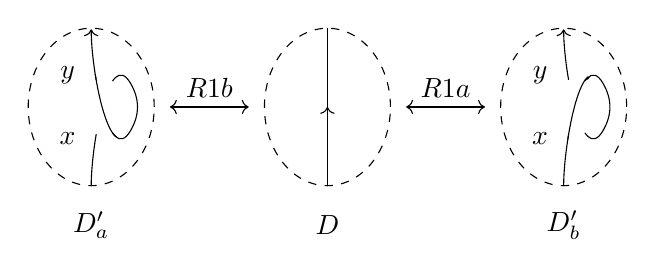
\begin{tikzpicture}
    \draw[->] (0, 0)--(0, 1);
    \draw (0, 1)--(0, 2);
    \draw[dashed] (0, 1) ellipse (0.8 and 1);

    \begin{knot}[
        consider self intersections,
        ignore endpoint intersections=false,
        flip crossing=1,
        clip width=20pt
      ]
      \strand[->] (-3, 0) to[out=90, in=120] (-2.5, 1.3) to[out=-60, in=60] (-2.5, .7) to[out=-120, in=-90] (-3, 2);
    \end{knot}
    \draw[dashed] (-3, 1) ellipse (0.8 and 1);

    \draw[dashed] (3, 1) ellipse (0.8 and 1);
    \begin{knot}[
        consider self intersections,
        ignore endpoint intersections=false,
        clip width=20pt
        %flip crossing=1
      ]
      \strand[->] (3, 0) to[out=90, in=120] (3.5, 1.3) to[out=-60, in=60] (3.5, .7) to[out=-120, in=-90] (3, 2);
    \end{knot}
    \node at (0, -.5) {$D$};
    \node at (3, -.5) {$D_b'$};
    \node at (-3, -.5) {$D_a'$};

    \node at (-3.3, .6) {$x$};
    \node at (-3.3, 1.4) {$y$};

    \node at (2.7, .6) {$x$};
    \node at (2.7, 1.4) {$y$};

    %\node at (.3, .6) {$w$};

    \draw[<->] (-2, 1)--(-1, 1) node[midway, above] {$R1b$};
    \draw[<->] (2, 1)--(1, 1) node[midway, above] {$R1a$};
  \end{tikzpicture}
\end{center}

Both Reidemeister moves $R1a$ and $R1b$ require the following diagram to commute,
\begin{center}
  \begin{tikzcd}
    M^{s+1}\arrow[r, "D'\phi"]\arrow[d, twoheadrightarrow] & N^{x+1} \arrow[d, twoheadrightarrow] \\ 
    M^{s+1},\; x=y \arrow[d, "f" left] & N^x\oplus (N/\phi_\pm(M^3)) \arrow[d, "g"] \\ 
    M^s \arrow[r, "D\phi" below] & N^x
  \end{tikzcd}
\end{center}
where $\phi_\pm$ changes (for $R1a$ we have $+$ and for $R1b$ $-$). We take $f$ and $g$ to be given by
$$f(m_1,..., m_s, m_{s+1})=(m_1,..., m_s+m_{s+1})$$
$$g(n_1,..., n_x, n_{x+1})=(n_1,..., n_x+n_{x+1}).$$
The homomorphism $f$ ensures that on the rest of diagrams $D'$ arc labeled $x$ in figure above and $y$ add up to the arc visible in the diagram $D$. Meanwhile, $g$ ensures that the additional crossing is treated with the appropriate coloring rule.

In terms of matrices, the above diagram can be translated to
$$
\begin{matrix}
  D_a' & & D & & D_b'\\ 
  \begin{bmatrix}
    %&X & Y & \hdots\\ 
    b & a+c  & 0 & \hdots\\ 
    x_1 & y_1 & z_1 \\ 
    \vdots & & & \ddots
  \end{bmatrix} 
       & \overset{R1a}{\sim} &
     \begin{bmatrix}
       x_1 + y_1 & z_1 & \hdots\\ 
       \vdots & & \ddots
     \end{bmatrix} 
       & \overset{R1b}{\sim} &
  \begin{bmatrix}
    %&X & Y & \hdots\\ 
    \beta & \alpha+\gamma  & 0 & \hdots\\ 
    x_1 & y_1 & z_1 \\ 
    \vdots & & & \ddots
  \end{bmatrix} 
\end{matrix}
$$
where $(\forall\;i=1,...,x)\;x_i=0\;\lor y_i=0$.

\subsection*{\centering R2}

\begin{center}
  \begin{tikzpicture}
    \draw[dashed] (0, 0) ellipse (.8 and 1);
    \draw[dashed] (3, 0) ellipse (.8 and 1);

    \begin{knot}[
      % draft mode=crossings, 
      clip width = 4pt,
      flip crossing=1,
      flip crossing=2, 
      % ignore endpoint intersection=false
      ]
      \strand[->] (-75:.8 and 1) to [out=90, in=-90] (0, 0) to[out=90, in=-90] (75:.8 and 1);
      \strand[->] (-105:.8 and 1) to [out=90, in=-90] 
      (.35, 0) to [out=90, in=-90]
      (105:.8 and 1);
    \strand[->] ($(3, 0)+(-75:.8 and 1)$) -- ($(3, 0)+(75:.8 and 1)$);
    \strand[->] ($(3, 0)+(-105:.8 and 1)$) -- ($(3, 0)+(105:.8 and 1)$);
    \end{knot}

    \node at (-.2, -1.5) {$D'$};
    \node at (3, -1.5) {$D$};

    \node at (-.4, 0) {$y$};
    \node at (75:1 and 1.3) {$z$};
    \node at (-75:1 and 1.3) {$x$};
  \end{tikzpicture}
\end{center}

For the second Reidemeister move we will say that $D\phi$ and $D'\phi$ are in relation if the following diagram commutes:

\begin{center}
  \begin{tikzcd}
    M^{s+2}\arrow[r, "D'\phi"]\arrow[d, twoheadrightarrow] & N^{x+2} \arrow[d, twoheadrightarrow] \\ 
    M^{s+2}, x=z\arrow[d] & N^x\oplus (N/\phi_{\pm}(M^3))\oplus (N/\phi_\mp(M^3))\arrow[d]\\ 
    M^s\arrow[r, "D\phi" ] & N^x
  \end{tikzcd}
\end{center}

In terms of matrices, the following move is admitted:

$$
\begin{matrix}
  D' & D \\ 
  \begin{bmatrix} 
    b & c & 0 & a & \hdots \\ 
    0 & \beta & \gamma &\alpha \\ 
    x_1 & 0 & z_1 & w_1 \\ 
    \vdots & & & &\ddots
  \end{bmatrix} 
     & \begin{bmatrix} 
       x_1+z_1 & w_1 & \hdots \\ 
       \vdots & & \ddots
     \end{bmatrix}
\end{matrix}
$$
where $(\forall\; i=1,...,x)\;x_i=0\;\lor z_i=0$.

\subsection*{\centering R3}

\begin{center}
  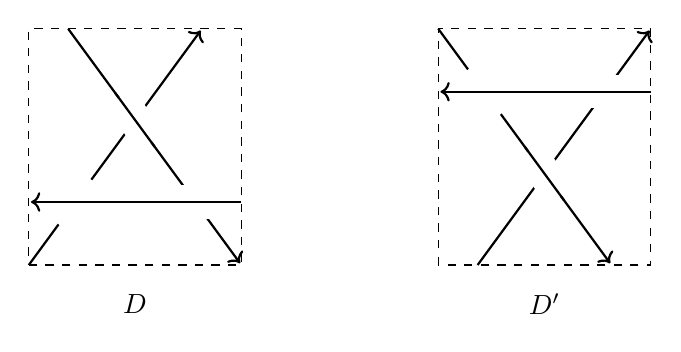
\begin{tikzpicture}
    \begin{knot}[
      % draft mode=crossings, 
      clip width=15pt, 
      flip crossing=1, 
      flip crossing = 2, 
      flip crossing=3, 
      flip crossing=4, 
      flip crossing=6, 
      flip crossing=5
      ]
            \strand[->, thick] (3.8, -5)--(6, -2);
      \strand[->, thick] (4.3, -2)--(6.5, -5);
      \strand[<-, thick] (3.8, -4.2)--(6.5, -4.2);

      \strand[->, thick] (9.5, -5)--(11.7, -2);
      \strand[->, thick] (9, -2)--(11.2, -5);
      \strand[<-, thick] (9, -2.8)--(11.7, -2.8);
    \end{knot}

    \draw[dashed] (3.8, -5)--(6.5, -5)--(6.5, -2)--(3.8, -2)--cycle;
    \draw[dashed] (9, -5) rectangle (11.7, -2);
    
    \node at ( 6.5/2 + 3.8/2, -5.5) {$D$};
    \node at (9/2+11.7/2, -5.5) {$D'$};
  \end{tikzpicture}
\end{center}

{\large\color{purple}DOKOŃCZYĆ - czy tutaj komutujacy diagram cos da? znaczy w sumie to da, ale to jest jakies dzikie zamienianie wspolrzednych}

In terms of matrices, the following move is admitted: 

$$
\begin{matrix}
  D' & D \\ 
  \begin{bmatrix}
    \alpha & \gamma & \beta & 0 & 0 & 0 & \hdots \\ 
    0 & 0 & c & b & 0 & a \\ 
    \beta & 0 & 0 & 0 & \gamma & \alpha \\ 
    u_1 & 0 & v_1 & w_1 & x_4 & y_4 \\ 
    \vdots & & & & & & \ddots
  \end{bmatrix}
     & 
  \begin{bmatrix}
    0 & 0 & \gamma & \beta & \alpha & 0 & \hdots  \\ 
    \beta & 0 & 0 & 0 & \gamma & \alpha \\ 
    0 & c & b & 0 & 0 & a\\ 
    u_4 & 0 & v_4 & w_4 & x_4 & y_4\\ 
    \vdots & & &  & & \ddots
  \end{bmatrix}
\end{matrix}
$$

\begin{theorem}
  The equivalence class of a color checking matrix of a diagram $D\phi$ under relation generated by matrix relations $R1a$, $R1b$, $R2$ and $R3$ is a knot diagram. Thus we can define $K\phi:=[D\phi]$.
\end{theorem}

\begin{proof}
  A direct result of the definition of the equivalence relation.
\end{proof}


\subsection{Reduced Smith normal form}

\input{rozdzialy/03-04-reduced-smith-normal.tex} 


% \section{Category of palettes}

% \subsection{Palettes}

We will work towards defining a category of palettes for a chosen knot $K$. This will allow us to change rules of colorings as we see fit.

\begin{definition}[palette]
  Let $R$ be a commutative ring with unity, $M$ a finitely generated $R$-module and $\mathcal{C}\subseteq M^3\oplus M^3$ to be a coloring rule confomring to all rules outlined in the previous section. We say that a triplet $(R, M, \mathcal{C})$ is a \buff{palette}.
\end{definition}

Notice that if there is a ring homomorphism $f:R\to S$ then we can consider $M$ as a $S$ module by tensoring with $S$. This allows us to write a morphism between palettes
$$\overline{f}:(R, M, \mathcal{C})\to (S, M_S, \mathcal{C}_S).$$
Similarly, if there is a module homomorphism $g:M\to M'$, then the induced morphism of palettes is
$$\overline{g}:(R, M, \mathcal{C})\to (R, M', \mathcal{C}').$$

\begin{definition}[category of palettes for knot $K$]
  We define $\Col(K)$ to be a \buff{category of palettes} of $K$ with 
  $$\text{Ob}(\Col(K))=\{(R, M, \mathcal{C})\}$$
  being all palettes as described above and for any two palettes
  $$\Hom((R, M, \mathcal{C}), (S, N, \mathcal{K}))$$
  is the set of induced morphisms $\overline{g}$ between modules or $\overline{f}$ between rings, when modules are $M$ and $N=M_S$ respectively.
\end{definition}

It is beneficial to highlight one palette in particular: 
$${(\Z[\Z], \Z[\Z], \{(u, i, (1-t)u+ti)\;:\;u,i\in\Z[\Z]\})},$$
which will be referred to as the \buff{Alexander palette}. We can derive this palette (which was used in \cref{example reduced normal form}) from the Wirtinger presentation of a knot as follows.

Consider a crossing
\begin{center}
  \begin{tikzpicture}
    \draw[<-] (0, 0) node[above] {$o$} --(2, 0) node[above] {$i$};
    \fill[white](1, 0) circle (7pt);
    \draw[->] (1, -1) node[right] {$u$}--(1, 1);
  \end{tikzpicture}
\end{center}
and take some $x$ to be the generator that is used to generate a representation for $K_G^{ab}$. Then, the following is a relation in said group:
$$UxCx(Ux)^{-1}=Ix$$
where $U=ux^{-1}$, $I=ix^{-1}$ and $O=ox^{-1}$. 
We can multiply both sides by $x^{-1}$ to obtain
$$x^{-1}UxCU^{-1}=x^{-1}Ix$$
which is change in $\Z[\Z]$ to
$$
tU+C-U=tI\implies 0=(1-t)U+tI-C
$$
The procedure for the other type of crossing is analogous.

The question that presents itself here is whether using row and column operations one can obtain representation matrix for the Alexander module from coloring matrices.



% Fixing the ring $R$ hints at $(R, 0, 0)$ being a trivial palette and products and coproducts of palettes being defined by their modules:
% $$(R, M, \mathcal{C})\oplus (R, N, \mathcal{K}):=(R, M\oplus N, \mathcal{C}\oplus \mathcal{K}).$$
%
% % \begin{conjecture}
% %   A category of palettes over a fixed ring $R$, $\mathcal{Col}_R(K)$ is Abelian.
% % \end{conjecture}
%
%
%



\bibliographystyle{jae}
\bibliography{literatura}

\newpage 



% \section{Index of notation}
%
% \begin{multicols}{2}
%   \begin{itemize}
%     \item[$K$] a knot with $s$ segments and $x$ crossings 
%     \item[$D$] a diagram of knot $K$
%     \item[$G$] the knot group of $K$
%     \item[$K_G$] knot or the kernel of the abelianization of the knot group
%     \item[$A_D$] Alexander matrix of $G$ using Wirtinger presentation from diagram $D$
%   \end{itemize}
% \end{multicols}
%
%
\end{document}
